\documentclass[tikz]{standalone}
\usepackage{tikz}
\usetikzlibrary{arrows.meta, calc, positioning}

\begin{document}
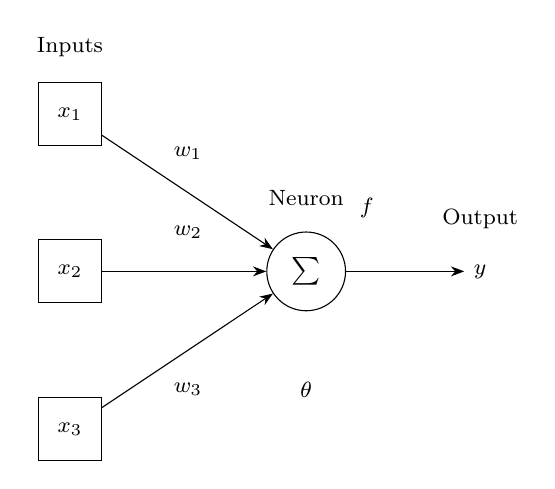
\begin{tikzpicture}[
  >=Stealth,
  neuron/.style={circle, draw, minimum size=1cm},
  input/.style={rectangle, draw, minimum size=0.8cm},
  every node/.style={font=\footnotesize}
]

% Input nodes
\node[input] (x1) at (-3,2) {$x_1$};
\node[input] (x2) at (-3,0) {$x_2$};
\node[input] (x3) at (-3,-2) {$x_3$};

% Neuron
\node[neuron] (n) at (0,0) {$\sum$};

% Weights
\node (w1) at (-1.5,1.5) {$w_1$};
\node (w2) at (-1.5,0.5) {$w_2$};
\node (w3) at (-1.5,-1.5) {$w_3$};

% Threshold
\node (theta) at (0,-1.5) {$\theta$};

% Output
\node[right=1.5cm of n] (y) {$y$};

% Connections
\draw[->] (x1) -- (n);
\draw[->] (x2) -- (n);
\draw[->] (x3) -- (n);
\draw[->] (n) -- (y);

% Activation function
\node[above right=0.2cm and 0.2cm of n] {$f$};

% Labels
\node[above=0.2cm of x1] {Inputs};
\node[above=0.2cm of n] {Neuron};
\node[above=0.2cm of y] {Output};

\end{tikzpicture}
\end{document}